\chapter{Tecniche crittografiche classiche}
\section{Modelli di crittografia simmetica}
La crittografia simmetrica è formata da cinque elementi:
\begin{itemize}
    \item \textbf{Plaintext}: si tratta del testo in chiaro, quindi interpretabile.
    \item \textbf{Algoritmo di cifratura}: l'algoritmo di cifratura esegue 
    varie sostituzioni e trasformazioni del testo in chiaro.
    \item \textbf{Chiave segreta}: la chiave è anch'essa argomento dell'algoritmo 
    di cifratura. La chiave è indipendente dal testo in chiaro e dall'algoritmo. 
    L'algoritmo produrrà un risultato diverso a seconda della specifica chiave utilizzata.
    \item \textbf{Testo cifrato}: Si tratta del messaggio prodotto in output. Dipenderà 
    dal testo in chiaro e dalla chiave segreta. Date due chiavi diverse il risultato 
    in output sarà diverso, genererà quindi due testi cifrati differenti. Il testo 
    cifrato è apparentemente un flusso di dati casuale, sarà quindi illegibile.
    \item \textbf{Algoritmo di decifratura} Si tratta essenzialmente dell'algoritmo 
    di cifratura eseguito inversamente. Prende in input il testo cifrato e la chiave, producendo 
    il testo originale.
\end{itemize}
Ci sono due requisiti per per l'uso sicuro della crittografia convenzionale:
\begin{enumerate}
    \item Abbiamo bisogno di un'algoritmo di cifratura forte. Ciò significa che 
    che chi possiede testi cifrati non sia in grado di trovare facilmente la chiave per
    poterli decifrare.
    \item Il mittente e il destinatario devono aver ricevuto le copie delle chiavi 
    segrete mediante un canale sicuro. Se qualcuno trovasse la chiave conoscendo 
    l'algoritmo, l'intera comunicazione diventerebbe leggibile.
\end{enumerate}
Nella cifratura simmetrica, l'algoritmo di cifratura non deve rimanere segreto, 
ma solo la chiave. Questa caratteristica la rende pratica per un uso diffuso.
I chip di cifratura a basso costo sono ampiamente disponibili e incorporati
in vari prodotti. La principale preoccupazione di sicurezza è mantenere
segreta la chiave.
\subsection{Elementi essenziali di una cifratura simmetrica}
\begin{itemize}
    \item Una sorgente produce un messaggio in testo in chiaro $X = [X_1, X_2, \ldots, X_M]$.
    \item Viene generata una chiave di cifratura $K = [K_1, K_2, \ldots, K_J]$, che deve essere mantenuta segreta.
    \item Con il messaggio $X$ e la chiave $K$ come input, l'algoritmo di cifratura genera 
    il testo cifrato $Y = [Y_1, Y_2, \ldots, Y_N]$, rappresentato come $Y = E(K, X)$.
    \item Il destinatario inteso, in possesso della chiave, può decifrare il messaggio: $X = D(K, Y)$.
\end{itemize}

\subsection{Sicurezza}
Un avversario che osserva $Y$ senza conoscere $K$ o $X$ può tentare di recuperare $X$ o $K$. 
È presumibile che l'avversario conosca gli algoritmi di cifratura (E) e decifratura (D).
Se l'avversario è interessato solo a un messaggio specifico, si concentrerà sul recupero
di $X$. Tuttavia, se desidera leggere futuri messaggi, cercherà di recuperare $K$.

\subsection{Crittografia}
I sistemi crittografici possono essere caratterizzati lungo tre dimensioni
indipendenti:
\begin{enumerate}
    \item \textbf{Il tipo di operazioni utilizzate per trasformare il testo in chiaro
    in testo cifrato}. Tutti gli algoritmi di cifratura si basano su due principi
    generali: la sostituzione, in cui ciascun elemento nel testo in 
    chiaro (\textit{bit, lettera, gruppo di bit o lettere}) è mappato
    in un altro elemento, e la trasposizione, in cui gli elementi nel
    testo in chiaro vengono riarrangiati. Il requisito fondamentale è
    che non venga persa alcuna informazione (\textit{ossia, che tutte
    le operazioni siano reversibili}). La maggior parte dei sistemi,
    chiamati sistemi a prodotto, coinvolge multiple fasi di sostituzioni
    e trasposizioni.
    \item \textbf{Il numero di chiavi utilizzate}. Se mittente e destinatario
    utilizzano la stessa chiave, il sistema è chiamato simmetrico,
    a chiave singola, a chiave segreta o cifratura convenzionale.
    Se mittente e destinatario utilizzano chiavi diverse, il sistema
    è chiamato asimmetrico, a due chiavi o cifratura a chiave pubblica.
    \item \textbf{Il modo in cui il testo in chiaro viene processato}. Una cifra
    a blocchi processa l'input un blocco di elementi alla volta, producendo
    un blocco di output per ciascun blocco in input. Una cifra a flusso
    processa gli elementi in input in modo continuo, producendo l'output
    elemento per elemento man mano che procede.
\end{enumerate}

Solitamente, l'obiettivo nell'attaccare un sistema di crittografia è di recuperare la chiave
in uso anziché semplicemente ottenere il testo in chiaro di un singolo testo cifrato. Esistono
due approcci generali per attaccare uno schema di crittografia convenzionale:

\begin{enumerate}
    \item \textbf{Criptoanalisi:} Gli attacchi crittoanalitici si basano sulla natura
    dell'algoritmo e talvolta su qualche conoscenza delle caratteristiche generali del
    testo in chiaro o anche su alcune coppie di testo in chiaro - testo cifrato di esempio.
    Questo tipo di attacco sfrutta le caratteristiche dell'algoritmo per cercare
    di dedurre un testo in chiaro specifico o la chiave in uso.
    \item \textbf{Attacco a Forza Bruta:} L'attaccante prova ogni possibile chiave su
    un testo cifrato finché non ottiene una traduzione intelligibile in testo in chiaro. In media,
    è necessario provare la metà di tutte le chiavi possibili per avere successo.
\end{enumerate}

Se uno dei due tipi di attacco riesce a dedurre la chiave, l'effetto è catastrofico:
tutti i messaggi futuri e passati crittografati con quella chiave sono compromessi.

Il primo tipo di attacco, la criptoanalisi, si basa sulla conoscenza dell'algoritmo
e delle caratteristiche del testo in chiaro o su coppie di testo in chiaro - testo cifrato di esempio.
L'obiettivo è dedurre il testo in chiaro o la chiave in uso. L'altro tipo di attacco è basato
sulla forza bruta, dove vengono provate tutte le possibili chiavi fino a trovare
una traduzione intelligibile del testo cifrato.

L'attacco basato solo sul testo cifrato è il più facile da difendere perché l'avversario
ha la minore quantità di informazioni con cui lavorare. Tuttavia, in molti casi,
l'analista dispone di più informazioni. L'analista potrebbe essere in grado di catturare
uno o più messaggi in testo in chiaro insieme alle loro cifrature. Oppure l'analista potrebbe
sapere che certi modelli di testo in chiaro appariranno in un messaggio. Ad esempio,
un file codificato in formato PostScript inizia sempre con lo stesso modello,
o potrebbe esserci un'intestazione o un banner standardizzato in un messaggio
di trasferimento di fondi e così via. Tutti questi sono esempi di testo in chiaro
conosciuti. Con questa conoscenza, l'analista potrebbe essere in grado di dedurre
la chiave in base al modo in cui il testo in chiaro noto viene trasformato.

Strettamente correlato all'attacco basato sul testo in chiaro conosciuto è quello
che potrebbe essere definito come un attacco basato su parole probabili.
Se l'avversario sta lavorando con la crittografia di un messaggio di prosa
generale, potrebbe avere poca conoscenza di ciò che è nel messaggio. Tuttavia,
se l'avversario sta cercando informazioni molto specifiche, potrebbero essere
noti alcuni pezzi del messaggio. Ad esempio, se viene trasmesso un intero
file contabile, l'avversario potrebbe conoscere la posizione di alcune parole
chiave nell'intestazione del file. Come altro esempio, il codice sorgente
di un programma sviluppato dalla Corporation X potrebbe includere una
dichiarazione di copyright in una posizione standardizzata. Se l'analista
è in grado in qualche modo di far inserire al sistema sorgente un messaggio
scelto dall'analista, allora è possibile un attacco basato sul testo in chiaro
scelto. Un esempio di questa strategia è la crittoanalisi differenziale.
In generale, se l'analista è in grado di scegliere i messaggi da cifrare,
potrebbe deliberatamente selezionare modelli che possono essere previsti
per rivelare la struttura della chiave.

Due altri tipi di attacco elencati sono testo cifrato scelto e testo scelto,
che sono meno comuni ma possibili. Solo algoritmi relativamente deboli non
resistono a un attacco basato solo sul testo cifrato. In generale, un algoritmo
di crittografia è progettato per resistere a un attacco basato sul testo in chiaro
conosciuto. Uno schema di crittografia è incondizionatamente sicuro se il
testo cifrato generato dallo schema non contiene informazioni sufficienti
per determinare univocamente il testo in chiaro corrispondente, indipendentemente
dalla quantità di testo cifrato disponibile. Cioè, non importa quanto tempo abbia
un avversario, è impossibile per lui o lei decifrare il testo cifrato
semplicemente perché le informazioni necessarie non ci sono. Con
l'eccezione di uno schema noto come ``one-time pad", non esiste
un algoritmo di crittografia che sia incondizionatamente sicuro.
Pertanto, tutto ciò a cui gli utenti di un algoritmo di crittografia
possono aspirare è un algoritmo che soddisfi una o entrambe delle
seguenti criteri:

\begin{enumerate}
    \item Il costo per rompere la cifra supera il valore delle informazioni
    crittografate.
    \item Il tempo richiesto per rompere la cifra supera la vita utile
    delle informazioni.
\end{enumerate}

Uno schema di crittografia è considerato sicuro computazionalmente se
soddisfa una qualsiasi delle due precedenti criteri. Sfortunatamente,
è molto difficile stimare la quantità di sforzo necessaria per
crittoanalizzare con successo il testo cifrato.

Tutte le forme di crittoanalisi per gli schemi di crittografia
simmetrica sono progettate per sfruttare il fatto che tracce di
struttura o modello nel testo in chiaro possono sopravvivere alla crittografia
e possono essere discernibili nel testo cifrato.
\section{Tecniche di sostituzione}
I due elementi base di tutte le tecniche di crittografia sono la sostituzione e 
la trasposizione.

Una tecnica di sostituzione è una tecnica in cui le lettere del testo in chiaro vengono 
sostituite da altre lettere o da numeri o simboli. Se il testo in chiaro 
viene visto come una sequenza di bit, allora la sostituzione comporta la sostituzione 
di modelli di bit del testo in chiaro con modelli di bit di testo cifrato.
\subsection{Cifrario di cesare}
Il cifrario di Cesare è noto come il primo e più semplice esempio di
cifrario a sostituzione. Fu utilizzato da Giulio Cesare e coinvolge la
sostituzione di ogni lettera dell'alfabeto con la lettera situata tre
posizioni più in basso nell'alfabeto. Ad esempio:

\begin{center}
\begin{tabular}{|c|c|}
\hline
\textbf{Plain} & \textbf{Ciphertext} \\
\hline
a & D \\
b & E \\
c & F \\
d & G \\
e & H \\
f & I \\
g & J \\
h & K \\
i & L \\
j & M \\
k & N \\
l & O \\
m & P \\
\hline
\end{tabular}
\hspace{2cm}
\begin{tabular}{|c|c|}
\hline
\textbf{Plain} & \textbf{Ciphertext} \\
\hline
n & Q \\
o & R \\
p & S \\
q & T \\
r & U \\
s & V \\
t & W \\
u & X \\
v & Y \\
w & Z \\
x & A \\
y & B \\
z & C \\
\hline
\end{tabular}
\end{center}

È importante notare che l'alfabeto è avvolto in modo che la lettera
successiva a Z sia A. Ogni lettera dell'alfabeto viene quindi sostituita
dalla lettera che si trova a tre posizioni più in basso.

Il cifrario di Cesare è un esempio semplice ma storico di crittografia a
sostituzione. Può essere utilizzato per crittografare un messaggio
spostando ogni lettera di tre posizioni nell'alfabeto.

L'algoritmo utilizzato è il seguente:
\[
C = E(3, p) = (p + 3)\mod 26  
\]
Lo shift potrebbe essere un valore generico $k$, quindi l'agoritmo generalizzato 
è:
\[
C = D(k, p) = (p + k)\mod 26  
\]
ove $k$ prende un valore nel compreso tra $1$ e $25$. L'algoritmo di 
decifrazione è simile:
\[
  p = D(k, C) = (C - k)\mod 26  
\]

Se è noto che un certo testo cifrato è un cifrario di Cesare, allora 
una crittoanalisi a forza bruta è facilmente eseguibile: basta provare
tutte e 25 le possibili chiavi. La Figura 2.3 mostra i risultati di
questa strategia applicata all'esempio di ciphertext. In questo caso,
il plaintext salta fuori occupando la terza linea.

Tre importanti caratteristiche di questo problema ci hanno permesso
di utilizzare una crittoanalisi a forza bruta:
\begin{enumerate}
    \item Gli algoritmi di cifratura e decifratura sono noti.
    \item Ci sono solo $25$ chiavi da provare.
    \item La lingua del plaintext è nota ed è facilmente riconoscibile.
\end{enumerate}

La crittoanalisi a forza bruta è un metodo efficace quando si tratta
di cifrari di Cesare, in quanto le limitate possibilità di chiavi e
la conoscenza dell'algoritmo semplificano notevolmente il processo
di decrittografia.

Nella maggior parte delle situazioni di networking, possiamo presumere
che gli algoritmi siano noti. Quello che rende generalmente impraticabile
la crittoanalisi a forza bruta è l'uso di un algoritmo che impiega un
grande numero di chiavi. Ad esempio, l'algoritmo Triple DES, esaminato
nel Capitolo 6, utilizza una chiave di 168 bit, che crea uno spazio
delle chiavi di $2^{168}$ o più di $3.7 \times 10^{50}$ possibili
chiavi.

La terza caratteristica è anche significativa. Se la lingua del
plaintext è sconosciuta, allora l'output del plaintext potrebbe non
essere riconoscibile. Inoltre, l'input potrebbe essere abbreviato o
compresso in qualche modo, rendendo di nuovo difficile il riconoscimento.
\subsection{Cifrario  monoalfabetico}
Con solo 25 chiavi possibili, il cifrario di Cesare è molto lontano
dall'essere sicuro. Un aumento drammatico dello spazio delle chiavi
può essere ottenuto consentendo una sostituzione arbitraria. Prima
di procedere, definiamo il termine ``permutazione".
\begin{tcolorbox}[title = {Permutazione}]
Una permutazione di un insieme finito di elementi $S$ è una
sequenza ordinata di tutti gli elementi di $S$, con ciascun elemento
che appare esattamente una volta. Ad esempio, se $S = \{a, b, c\}$, ci
sono sei permutazioni di $S$:
\end{tcolorbox}
\[
abc, acb, bac, bca, cab, cba
\]
In generale, ci sono $n!$ permutazioni di un insieme
di $n$ elementi, poiché il primo elemento può essere scelto in uno
dei modi $n$ possibili, il secondo in $n - 1$ modi, il terzo
in $n - 2$ modi e così via.

Ricordiamo l'assegnazione per il cifrario di Cesare:
\begin{center}
\begin{tabular}{|c|c|}
\hline
\textbf{Plain} & \textbf{Ciphertext} \\
\hline
a & D \\
b & E \\
c & F \\
d & G \\
e & H \\
f & I \\
g & J \\
h & K \\
i & L \\
j & M \\
k & N \\
l & O \\
m & P \\
\hline
\end{tabular}
\end{center}

Se invece la linea ``ciphertext" può essere qualsiasi permutazione
dei $26$ caratteri alfabetici, allora ci sono $26!$ o più di $4 \times 10^{26}$
possibili chiavi. Questo è $10$ ordini di grandezza superiore all
spazio delle chiavi per \verb|DES| e sembrerebbe eliminare le tecniche di
crittoanalisi a forza bruta. Un approccio del genere è chiamato
cifrario di sostituzione monoalfabetica, perché viene utilizzato
un singolo alfabeto cifrato (\textit{mappatura dall'alfabeto in chiaro
all'alfabeto cifrato}) per ogni messaggio.

C'è, tuttavia, un'altra linea di attacco. Se il crittoanalista
conosce la natura del testo in chiaro (\textit{ad esempio, testo inglese
non compresso}), può sfruttare le regolarità della lingua. Per vedere
come potrebbe procedere tale crittoanalisi, diamo qui un esempio
parziale adattato da uno in \verb|[SINK09]|. Il testo cifrato da
risolvere
è il seguente:
\begin{verbatim}
UzqSovUoHxmoPvgPozPevSgzWSzoPfPeSxUDBmeTSxaIz
vUePHzHmDzSHzoWSfPaPPDTSvPqUzWymxUzUHSx
ePyePoPDzSzUfPomBzWPfUPzHmDJUDTmoHmq
\end{verbatim}
Come primo passo, può essere determinata la frequenza relativa delle
lettere e confrontata con una distribuzione di frequenza standard per
l'inglese.
Se il messaggio fosse abbastanza lungo, questa tecnica da sola potrebbe
essere sufficiente, ma poiché questo è un messaggio relativamente breve,
non possiamo aspettarci una corrispondenza esatta. In ogni caso, le
frequenze relative delle lettere nel testo cifrato (\textit{in percentuale}) sono
le seguenti:
\begin{figure}[H]
    \centering
    \begin{tabular}{cccc}
        P 13.33 & Z 11.67 & S 8.33 & U 8.33 \\
        O 7.50 & M 6.67 & H 5.83 & D 5.00 \\
        E 5.00 & V 4.17 & X 4.17 & F 3.33 \\
        W 3.33 & Q 2.50 & T 2.50 & A 1.67 \\
        B 1.67 & G 1.67 & Y 1.67 & I 0.83 \\
        J 0.83 & C 0.00 & K 0.00 & L 0.00 \\
        N 0.00 & R 0.00 &
    \end{tabular}
\end{figure}
confrontando questa suddivisione con la Figura \ref{fig:frequenza-lettere-testo-cifrato}, sembra probabile
che le lettere cifrate P e Z siano equivalenti alle lettere in chiaro e e t, ma non è certo quale sia
quale. Le lettere S, U, O, M e H sono tutte di frequenza relativamente alta e probabilmente corrispondono
alle lettere in chiaro dell'insieme \{\textit{a, h, i, n, o, r, s}\}. Le lettere con le frequenze più basse
(\textit{ovvero A, B, G, Y, I, J}) sono probabilmente incluse nell'insieme \{\textit{b, j, k, q, v, x, z}\}.

Ci sono diverse modalità per procedere in questo punto. Potremmo fare alcune assegnazioni
provvisorie e iniziare a completare il testo in chiaro per vedere se assomiglia a uno scheletro
ragionevole di un messaggio. Un approccio più sistematico è cercare altre regolarità. Ad esempio,
potrebbero essere noti alcuni termini nel testo. Oppure potremmo cercare sequenze ripetute di lettere
cifrate e cercare di dedurne le corrispondenti lettere in chiaro.

Un potente strumento è rappresentato dalla frequenza delle combinazioni di due lettere, note come digrammi.
Potrebbe essere compilata una tabella simile alla Figura \ref{fig:frequenza-lettere-testo-cifrato} che mostri
la frequenza relativa dei digrammi. Il digramma più comune è th. Nel nostro testo cifrato, il digramma più
comune è ZW, che appare tre volte. Quindi facciamo corrispondere Z a t e W a h. Quindi, in base alla nostra
ipotesi precedente, possiamo equiparare P a e. Ora notiamo che la sequenza ZWP appare nel testo cifrato, e possiamo
tradurre quella sequenza come ``the''. Questo è il trigramma (\textit{combinazione di tre lettere}) più frequente in inglese,
il che sembra indicare che siamo sulla strada giusta.

Successivamente, notiamo la sequenza ZWSZ nella prima riga. Non sappiamo se queste quattro lettere formano una
parola completa, ma se lo fanno, è del tipo $th\_t$. In tal caso, S corrisponde ad a.

\begin{figure}[H]
    \centering
    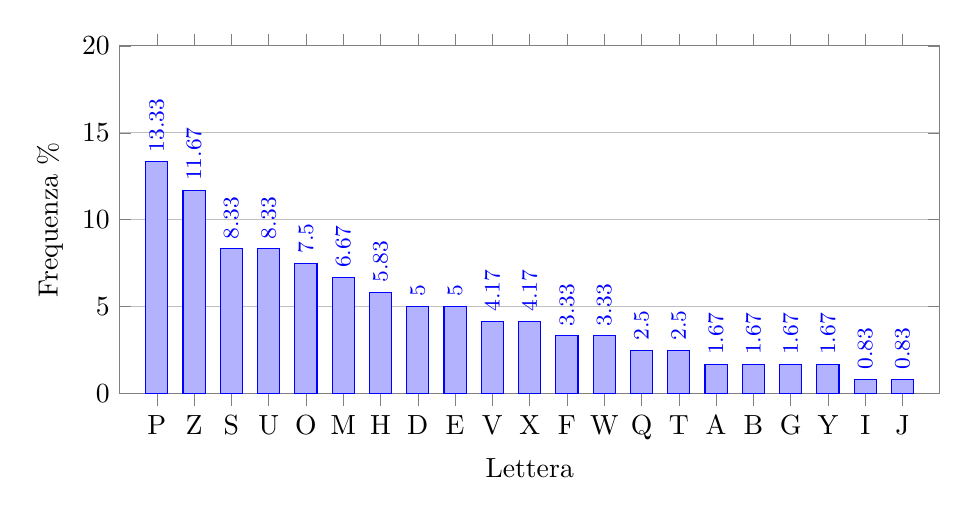
\begin{tikzpicture}
        \begin{axis}[
            ybar,
            ylabel=Frequenza \%,
            xlabel=Lettera,
            symbolic x coords={P, Z, S, U, O, M, H, D, E, V, X, F, W, Q, T, A, B, G, Y, I, J},
            xtick=data,
            nodes near coords,
            nodes near coords align={vertical}, % Imposta l'allineamento verticale dei numeri delle coordinate
            nodes near coords style={rotate=90}, % Ruota i numeri delle coordinate in verticale
            nodes near coords style={right, font=\footnotesize}, % Posiziona i numeri sopra le barre e riduce la dimensione del carattere
            width=12cm,
            height=6cm,
            enlarge x limits=0.05,
            ymin=0,
            ymax=20,
            ymajorgrids=true,
            bar width=8pt, % Larghezza delle barre
            axis line style={gray}, % Imposta il colore dell'asse su grigio
            y axis line style={gray}, % Imposta il colore dell'asse y su grigio
        ]
        \addplot coordinates {
            (P,13.33)
            (Z,11.67)
            (S,8.33)
            (U,8.33)
            (O,7.50)
            (M,6.67)
            (H,5.83)
            (D,5.00)
            (E,5.00)
            (V,4.17)
            (X,4.17)
            (F,3.33)
            (W,3.33)
            (Q,2.50)
            (T,2.50)
            (A,1.67)
            (B,1.67)
            (G,1.67)
            (Y,1.67)
            (I,0.83)
            (J,0.83)
        };
        \end{axis}
        \end{tikzpicture}
        \caption{Frequenze relative alle lettere nei testi inglesi}
        \label{fig:frequenza-lettere-testo-cifrato}
\end{figure}
Finora abbiamo identificato solo quattro lettere, ma già abbiamo una buona parte del messaggio.
Continuando l'analisi delle frequenze e sperimentando, dovremmo facilmente trovare una soluzione
da questo punto. Il testo completo, con spazi aggiunti tra le parole, è il seguente:

\begin{verbatim}
    it was disclosed yesterday that several informal but
    direct contacts have been made with political
    representatives of the viet cong in moscow
\end{verbatim}

I cifrari monoalfabetici sono facili da decifrare perché riflettono i dati di frequenza
dell'alfabeto originale. Una contromisura consiste nel fornire più sostituti, noti come omofoni,
per una singola lettera. Ad esempio, la lettera "e" potrebbe essere assegnata a diversi simboli
cifrati, come 16, 74, 35 e 21, con ciascun omofono assegnato a una lettera in rotazione o casualmente.
Se il numero di simboli assegnati a ciascuna lettera è proporzionale alla frequenza relativa di
quella lettera, le informazioni sulla frequenza delle singole lettere vengono completamente oscurate.
Il grande matematico Carl Friedrich Gauss credeva di aver ideato un cifrario infrangibile utilizzando
gli omofoni. Tuttavia, anche con gli omofoni, ogni elemento del testo in chiaro influenza
solo un elemento del testo cifrato, e i modelli di lettere multiple (\textit{ad esempio, le frequenze
dei digrammi}) sopravvivono comunque nel testo cifrato, rendendo la crittoanalisi relativamente semplice.

\subsection{Cifrario di Playfair}
Il cifrario di crittografia a più lettere più conosciuto è il cifrario di
\textit{Playfair}, che tratta i digrammi nel testo in chiaro come unità singole e li traduce
in digrammi nel testo cifrato. L'algoritmo di \textit{Playfair} si basa sull'uso di una matrice $5 \times 5$
di lettere costruita utilizzando una parola chiave. Ecco un esempio, risolto da Lord Peter Wimsey nel
romanzo ``Have His Carcase" di \textit{Dorothy Sayers}:

\begin{center}
    \begin{tikzpicture}[font=\ttfamily\small]
        \matrix (playfair) [matrix of nodes,nodes={draw,minimum size=12mm,anchor=center},column sep=-\pgflinewidth,row sep=-\pgflinewidth]{
            |[fill=gray!20]| M & |[fill=gray!20]| O & |[fill=gray!20]| N & |[fill=gray!20]| A & |[fill=gray!20]| R \\
            |[fill=gray!20]| H & |[fill=gray!20]| Y & B & C & D \\
            E & F & G & I & K \\
            L & P & Q & S & T \\
            U & V & W & X & Z \\
        };
      \end{tikzpicture}
    \end{center}
In questo caso, la parola chiave è "monarchia". La matrice viene costruita riempiendo le lettere della parola chiave (senza duplicati) da sinistra a destra e dall'alto verso il basso, e poi riempiendo il resto della matrice con le lettere rimanenti in ordine alfabetico. Le lettere I e J contano come una sola lettera. Il testo in chiaro viene crittografato due lettere alla volta, secondo le seguenti regole:
\begin{enumerate}
    \item Le lettere ripetute nel testo in chiaro che si trovano nella stessa coppia 
    vengono separate da una lettera di riempimento, come ad esempio ``x", quindi ``balloon" 
    verrebbe trattato come ``ba lx lo on".
    \item Due lettere nel testo in chiaro che si trovano nella stessa riga della matrice
    vengono ciascuna sostituite dalla lettera a destra, con il primo elemento della riga
    che segue ciclicamente l'ultimo. Ad esempio, ``ar" viene crittografato come ¡¡RM".
    \item Due lettere nel testo in chiaro che si trovano nella stessa colonna vengono ciascuna
    sostituite dalla lettera sottostante, con l'elemento superiore della colonna che segue
    ciclicamente l'ultimo. Ad esempio, ``mu" viene crittografato come ``CM".
    \item In caso contrario, ogni lettera nel testo in chiaro nella coppia viene sostituita
    dalla lettera che si trova nella stessa riga e nella colonna occupata dall'altra lettera
    nel testo in chiaro. Quindi, ``hs" diventa ``BP" e "ea" diventa ``IM" (o ``JM", a discrezione
    dell'incifratore).
\end{enumerate}
Il cifrario Playfair rappresenta un grande passo avanti rispetto ai semplici cifrari monoalfabetici.
Per una cosa, mentre ci sono solo $26$ lettere, ci sono 26 $\cdot 26 = 676$ digrammi, rendendo
più difficile l'identificazione dei digrammi individuali. Inoltre, le frequenze relative delle singole
lettere mostrano una gamma molto più ampia rispetto a quella dei digrammi, rendendo l'analisi delle
frequenze molto più difficile. Per queste ragioni, il cifrario Playfair è stato a lungo considerato
indistruttibile. È stato utilizzato come sistema standard sul campo dall'Esercito Britannico durante
la Prima Guerra Mondiale e ha ancora goduto di un notevole utilizzo da parte dell'Esercito degli Stati
Uniti e altre forze alleate durante la Seconda Guerra Mondiale.
Nonostante questo livello di fiducia nella sua sicurezza, il cifrario Playfair è relativamente facile
da decifrare, perché lascia comunque gran parte della struttura della lingua in chiaro intatta. Di solito,
poche centinaia di lettere del testo cifrato sono sufficienti.
Un modo per rivelare l'efficacia del cifrario Playfair e di altri cifrari è mostrato nella Figura \ref{fig:playfair}.
La linea etichettata ``testo in chiaro" rappresenta una tipica distribuzione di frequenza dei $26$ caratteri
alfabetici (\textit{senza distinzione tra maiuscole e minuscole}) in un testo normale. Questa è anche la
distribuzione di frequenza di qualsiasi cifrario di sostituzione monoalfabetica, perché i valori di
frequenza per le singole lettere sono gli stessi, solo con lettere diverse sostituite alle lettere
originali. Il grafico è sviluppato nel seguente modo: il numero di occorrenze di ciascuna lettera nel
testo viene conteggiato e diviso per il numero di occorrenze della lettera più frequentemente utilizzata.
Utilizzando i risultati della Figura \ref{fig:frequenza-lettere-testo-cifrato}, vediamo che la
lettera ``e" è quella più frequentemente utilizzata.
Di conseguenza, "e" ha una frequenza relativa di $1$, ``t" di $9.056/12.702 \approx 0,72$, e così via.
I punti sull'asse orizzontale corrispondono alle lettere in ordine decrescente di frequenza.
La Figura \ref{fig:playfair} mostra anche la distribuzione di frequenza che si ottiene quando il testo viene
crittografato utilizzando il cifrario Playfair. Per normalizzare il grafico, il numero di occorrenze
di ciascuna lettera nel testo cifrato è stato nuovamente diviso per il numero di occorrenze della
lettera ``e" nel testo in chiaro. Il grafico risultante mostra quindi in che misura la distribuzione
di frequenza delle lettere, che rende facile risolvere i cifrari di sostituzione, sia mascherata dalla
crittografia. Se l'informazione sulla distribuzione di frequenza fosse totalmente nascosta nel processo
di crittografia, il grafico delle frequenze nel testo cifrato sarebbe piatto e l'analisi crittografica
utilizzando solo il testo cifrato sarebbe effettivamente impossibile. Come mostra la figura, il cifrario
Playfair ha una distribuzione più piatta rispetto al testo in chiaro, ma comunque rivela molta struttura
su cui un crittoanalista può lavorare. Il grafico mostra anche il cifrario Vigenère, discusso
successivamente. Le curve di Hill e Vigenère nel grafico si basano su risultati riportati in \verb|[SIMM93]|.
\begin{figure}[H]
    \centering
    \includegraphics[width=0.8\textwidth]{img/frequenza_playfair.png}
    \caption{Frequenza delle occorrenze delle lettere nel testo cifrato}
    \label{fig:playfair}
\end{figure}
\subsection{Cifrario poliafabetico}
Un altro modo per migliorare la semplice tecnica monoalfabetica è utilizzare
diverse sostituzioni monoalfabetiche man mano che si procede attraverso il
messaggio in chiaro. Il nome generico per questo approccio è cifrario di sostituzione
polialfabetica. Tutte queste tecniche hanno le seguenti caratteristiche in comune:

\begin{enumerate}
  \item Un insieme di regole di sostituzione monoalfabetica correlate viene utilizzato.
  \item Una chiave determina quale particolare regola viene scelta per una data trasformazione.
\end{enumerate}

\subsubsection{Cifrario di Vigenère}
Il cifrario di Vigenère è uno dei più noti e semplici cifrari polialfabetici.
In questo schema, l'insieme di regole di sostituzione monoalfabetica correlate consiste
nei $26$ cifrari di Cesare con spostamenti da $0$ a $25$. Ogni cifrario è indicato da una chiave
lettera, che è la lettera cifrata che sostituisce la lettera in chiaro ``a". Quindi, un
cifrario di Cesare con uno spostamento di 3 è indicato dalla chiave ``3".

Il cifrario di Vigenère può essere espresso nel seguente modo. Supponiamo una sequenza
di lettere in chiaro $P = p_0, p_1, p_2, \ldots, p_{n-1}$ e una chiave costituita dalla
sequenza di lettere $K = k_0, k_1, k_2, \ldots, k_{m-1}$, dove tipicamente $m \leq n$.
La sequenza di lettere cifrate $C = C_0, C_1, C_2, \ldots, C_{n-1}$ viene calcolata come segue:

\[
    C_i = (p_i + k_{i \mod m}) \mod 26
\]

Dove $i \mod m$ indica l'operazione di modulo. In altre parole, si somma la lettera in chiaro
$p_i$ con la corrispondente lettera chiave $k_{i \mod m}$ e il risultato è ridotto modulo $26$
per ottenere la lettera cifrata $C_i$.

La decrittografia è effettuata in modo simile:

\[
p_i = (C_i - k_{i \mod m}) \mod 26
\]

Per crittografare un messaggio, è necessaria una chiave lunga quanto il messaggio stesso. Di solito,
la chiave è una parola chiave ripetuta. Ad esempio, se la parola chiave è ``deceptive" e il messaggio
è ``we are discovered save yourself", la cifratura procede come segue:

\begin{align*}
\text{chiave:} & \quad \text{deceptivedeceptivedeceptive} \\
\text{in chiaro:} & \quad \text{wearediscoveredsaveyourself} \\
\text{cifrato:} & \quad \text{zIcvTWqngRzgvTWavzHcqyglmgJ}
\end{align*}

Espresso in forma di enumerazione alfabetica, il cifrario di Vigenère è il seguente:

\begin{table}[H]
    \centering
    \begin{tabular}{|c|cccccccccccccc|}
    \hline
    \textbf{key} & 3 & 4 & 2 & 4 & 15 & 19 & 8 & 21 & 4 & 3 & 4 & 2 & 4 & 15 \\
    \hline
    \textbf{plaintext} & 22 & 4 & 0 & 17 & 4 & 3 & 8 & 18 & 2 & 14 & 21 & 4 & 17 & 4 \\
    \hline
    \textbf{ciphertext} & 25 & 8 & 2 & 21 & 19 & 22 & 16 & 13 & 6 & 17 & 25 & 6 & 21 & 19 \\
    \hline
    \end{tabular}
\end{table}

\begin{table}[H]
    \centering
    \begin{tabular}{|c|ccccccccccccc|}
    \hline
    \textbf{key} & 19 & 8 & 21 & 4 & 3 & 4 & 2 & 4 & 15 & 19 & 8 & 21 & 4 \\
    \hline
    \textbf{plaintext} & 3 & 8 18 & 0 & 21 & 4 & 24 & 14 & 20 & 17 & 18 & 4 & 11 & 5 \\
    \hline
    \textbf{ciphertext} & 22 & 0 & 21 & 25 & 7 & 2 & 16 & 24 & 6 & 11 & 12 & 6 & 9 \\
    \hline
    \end{tabular}
\end{table}
La forza di questo cifrario è che ci sono molte lettere cifrate per ciascuna lettera in chiaro,
una per ciascuna lettera unica della parola chiave. Pertanto, le informazioni sulla frequenza delle
lettere sono oscurate. Tuttavia, non viene persa tutta la conoscenza della struttura del testo in chiaro.

Innanzitutto, supponiamo che l'avversario ritenga che il cifrato sia stato crittografato utilizzando
una sostituzione monoalfabetica o un cifrario di Vigenère. Si può effettuare un semplice test per
effettuare una determinazione. Se si utilizza una sostituzione monoalfabetica, le proprietà statistiche
del cifrato dovrebbero essere le stesse del linguaggio del testo in chiaro. Quindi, facendo riferimento
alla Figura \ref{fig:frequenza-lettere-testo-cifrato}, dovrebbe esserci una lettera del cifrato con una
frequenza relativa di circa il $12,7\%$,
una con circa il $9,06\%$, e così via. Se è disponibile solo un singolo messaggio per l'analisi, non
ci si aspetterebbe una corrispondenza esatta di questo piccolo campione con il profilo statistico del
linguaggio del testo in chiaro. Tuttavia, se la corrispondenza è vicina, possiamo assumere una
sostituzione monoalfabetica.

Se, d'altra parte, si sospetta un cifrario di Vigenère, il progresso dipende dalla determinazione della
lunghezza della chiave, come verrà visto tra un momento. Per ora, concentriamoci su come può essere
determinata la lunghezza della chiave. L'importante intuizione che porta a una soluzione è la seguente:
se due sequenze identiche di lettere in chiaro si verificano a una distanza che è un multiplo intero della
lunghezza della chiave, genereranno sequenze di cifrati identiche. Nell'esempio precedente, due istanze
della sequenza ``red" sono separate da nove posizioni dei caratteri. Di conseguenza, in entrambi i casi,
la ``r" è cifrata usando la lettera chiave ``e", la ``e" è cifrata usando la lettera chiave ``p", e la ``d" è
cifrata usando la lettera chiave ``t". Quindi, in entrambi i casi, la sequenza di cifrati è ``VTW".
Indichiamo ciò evidenziando le lettere pertinenti del cifrato e sfumando i numeri di cifrato rilevanti.

Un analista che osserva solo il cifrato rileverebbe le sequenze ripetute ``VTW" con uno spostamento di
9 e farebbe l'assunzione che la chiave sia lunga tre o nove lettere. L'apparizione di ``VTW" due volte
potrebbe essere casuale e potrebbe non riflettere lettere in chiaro identiche crittografate con lettere
chiave identiche. Tuttavia, se il messaggio è abbastanza lungo, ci saranno diverse sequenze di cifrati
ripetuti. Cercando fattori comuni negli spostamenti delle diverse sequenze, l'analista dovrebbe essere
in grado di fare una buona congettura sulla lunghezza della chiave.

La soluzione del cifrario ora dipende da un'importante intuizione. Se la lunghezza della chiave è ``m", 
il cifrario, in effetti, consiste di ``m" sostituzioni monoalfabetiche separate. Ad esempio, con la chiave
``DECEPTIVE", le lettere nelle posizioni $1, 10, 19$ e così via sono tutte crittografate con lo stesso
cifrario monoalfabetico. Quindi, possiamo utilizzare le conosciute caratteristiche di frequenza del
linguaggio del testo in chiaro per attaccare separatamente ciascuna delle sostituzioni monoalfabetiche.

La natura periodica della chiave può essere eliminata utilizzando una chiave non ripetitiva lunga quanto
il messaggio stesso. Vigenère ha proposto quello che viene chiamato un sistema autokey, in cui una chiave
è concatenata al testo in chiaro stesso per fornire una chiave in esecuzione. Nel nostro esempio:

\begin{table}[H]
    \centering
    \begin{tabular}{|c|c|c|}
    \hline
    \textbf{Chiave} & deceptivewearediscoveredsav \\
    \hline
    \textbf{Testo in chiaro} & wearediscoveredsaveyourself \\
    \hline
    \textbf{Cifrato} & zIcvTWqngKzeIIgaSxSTSlvvWla \\
    \hline
    \end{tabular}
\end{table}

Anche questo schema è vulnerabile all'analisi crittografica. Poiché la chiave e il testo in
chiaro condividono la stessa distribuzione di frequenza delle lettere, è possibile applicare
una tecnica statistica. Ad esempio, la lettera ``e" cifrata con ``e", come indicato in
Figura \ref{fig:frequenza-lettere-testo-cifrato}, ci si aspetta che si verifichi con una
frequenza di $(0,127)^2 \approx 0,016$, mentre la lettera ``t" cifrata con ``t" si verificherebbe
solo circa la metà delle volte. Queste regolarità possono essere sfruttate per raggiungere un'analisi
crittografica di successo.

\subsubsection{Cifraro di Vernam}
La difesa definitiva contro una crittoanalisi di questo tipo consiste nel scegliere una chiave
lunga quanto il testo in chiaro e che non abbia alcuna relazione statistica con esso. Un sistema
del genere fu introdotto da un ingegnere AT\&T di nome Gilbert Vernam nel 1918.

\begin{figure}[H]
    \centering
    \includegraphics[width=0.8\textwidth]{img/xor_logico.png}
    \caption{Schema di Vernam}
    \label{fig:vernam}
\end{figure}
Il suo sistema lavora con i dati binari (\textit{bit}) e utilizza l'operazione di \verb|XOR| logico:
\[
  c_i = p_i \oplus k_i  
\]

dove:
\begin{itemize}
    \item $c_i$ è l'$i$-esimo bit del testo cifrato
    \item $p_i$ è l'$i$-esimo bit del testo in chiaro
    \item $k_i$ è l'$i$-esimo bit della chiave
    \item $\oplus$ è l'operatore \verb|XOR| logico
\end{itemize}

L'operazione di \verb|XOR| logico è definita come segue:
\begin{table}[H]
    \centering
    \begin{tabular}{|c|c|c|}
    \hline
    \textbf{Input} & \textbf{Output} & \textbf{Descrizione} \\
    \hline
    0 & 0 & 0 $\oplus$ 0 = 0 \\
    \hline
    0 & 1 & 0 $\oplus$ 1 = 1 \\
    \hline
    1 & 0 & 1 $\oplus$ 0 = 1 \\
    \hline
    1 & 1 & 1 $\oplus$ 1 = 0 \\
    \hline
    \end{tabular}
\end{table}

L'essenza di questa tecnica risiede nel modo in cui viene costruita la chiave. Vernam 
ha proposto l'uso di una lunga striscia di nastro che alla fine ripeteva la chiave, quindi 
di fatto il sistema funzionava con una chiave molto lunga ma ripetitiva. Sebbene uno schema 
del genere, con una chiave lunga, presenti notevoli difficoltà crittografiche, può essere violato con
una quantità sufficiente di testo cifrato, l'uso di sequenze di testo in chiaro conosciute o probabili, o entrambe.
\subsection{One-Time Pad}
Il cifrario monouso, o \textit{one-time pad}, è un sistema di crittografia che utilizza una chiave
casuale di lunghezza uguale o maggiore del messaggio da crittografare. È un sistema di crittografia
perfetta, nel senso che il messaggio cifrato non può essere decifrato o violato senza conoscere la chiave.
\begin{itemize}
    \item \textbf{Chiave Casuale}: La chiave utilizzata nel cifrario monouso è una sequenza 
    casuale di bit o caratteri, lunga quanto il messaggio da crittografare. Essendo completamente casuale, 
    non contiene alcuna struttura o pattern riconoscibile.
    
    \item \textbf{Lunghezza della Chiave}: La chiave deve essere della stessa lunghezza del messaggio 
    in chiaro. Questo significa che ogni messaggio richiede una chiave diversa e della stessa lunghezza.
    
    \item \textbf{Unicità}: Ogni chiave è utilizzata una sola volta. Dopo essere stata usata per crittografare
    o decrittografare un messaggio, la chiave viene scartata e non viene mai riutilizzata.
    
    \item \textbf{Sicurezza Statistica}: La sicurezza del cifrario monouso deriva dalla sua totale casualità.
    Poiché la chiave è una sequenza casuale e unica per ogni messaggio, non esiste alcuna relazione statistica
    tra il testo cifrato e il testo in chiaro. Questo significa che il testo cifrato non fornisce alcuna
    informazione utile per violare il cifrario, rendendolo teoricamente indistruttibile.
\end{itemize}
Il cifrario monouso, noto come ``one-time pad" è considerato perfetto dal punto di vista statistico
e crittografico per due ragioni principali:

\begin{enumerate}
    \item \textbf{Casualità della Chiave:} La chiave nel cifrario monouso è una sequenza casuale di bit o caratteri.
    La casualità è fondamentale dal punto di vista statistico. In termini di probabilità, ogni bit o carattere nella
    chiave ha una probabilità del 50\% di essere $0$ o $1$ (\textit{in caso di bit}) o di essere una qualsiasi
    lettera nell'alfabeto (\textit{in caso di caratteri}). Questo fatto è rappresentato dalla distribuzione di
    probabilità uniforme.
   
    Formula della distribuzione uniforme per bit:
    \[ P(X = 0) = P(X = 1) = \frac{1}{2} \]

    Formula della distribuzione uniforme per caratteri:
    \[ P(X = x_i) = \frac{1}{n} \text{ per ogni } x_i \text{ nell'alfabeto di lunghezza } n \]

    Ad esempio, in un alfabeto di $26$ lettere, la probabilità di ciascuna lettera è $1/26$.

    Nel caso di una chiave di lunghezza $n$, la probabilità di una particolare sequenza di $n$ bit o caratteri
    è $1/2^n$ o $1/n^n$ rispettivamente. Poiché non vi è alcuna relazione nei bit o caratteri della chiave.

    \item \textbf{Unicità della Chiave:} Ogni chiave viene utilizzata una sola volta per crittografare
    o decrittografare un messaggio specifico e viene scartata dopo l'uso. Questo significa che non c'è alcuna
    relazione statistica tra il testo cifrato e il testo in chiaro. L'assenza di qualsiasi pattern o relazione
    è fondamentale dal punto di vista della teoria della probabilità.
\end{enumerate}
\section{Concatenazione di crittosistemi}
Una permutazione è un mapping iniettivo e suriettivo di un insieme in se stesso.
Una permutazione è una sostituzione che mappa ogni lettera dell'alfabeto in un'altra lettera.
Quindi:
\[
    \pi : \mathcal{A} \rightarrow \mathcal{A}
\]
sappiamo che è vulnerabile all'analisi delle frequenze, quindi possiamo applicare 
un sistema di concatenazione:
\[
  \pi_1 \circ \pi_2 \circ \pi_3 \circ \pi_4 \circ \pi_5  
\]
il problema è che la composizione di permutazioni è ancora una permutazione,
quindi è la stessa cosa chè l'eseguire un'unica permutazione $\pi$.
Varia quindi solo la rappresentazione della permutazione.
Per risolvere il problema serve un elemento aggiuntivo che non sia una permutazione,
ad esempio una trasposizione.
\section{Macchina a Rotori}
Una macchina a rotori è una macchina crittografica che sfrutta
la crittografia a sostituzione \textbf{polialfabetica}. La macchina è composta
da cilindri rotanti, ognuno con $26$ pin di input e $26$ pin di output,
ciascuno con connessioni interne che collegano input e output in modo
univoco. Un singolo cilindro crea una sostituzione monoalfabetica,
ruotando dopo ogni input, il che crea una sostituzione polialfabetica
con un periodo di $26$ caratteri.

La vera forza delle macchine a rotori emerge quando vengono utilizzati
più cilindri collegati in serie. Quando si preme un tasto, il cilindro
più vicino all'input ruota di una posizione, influenzando il successivo
e così via. Questa configurazione crea una vasta varietà di sostituzioni
alfabetiche, con un'enorme quantità di possibilità quando si utilizzano
più cilindri.

Questo schema crittografico rappresenta una sfida significativa per i
crittoanalisti poiché richiede un'enorme quantità di dati cifrati per
essere decifrato in modo significativo, rendendo molto difficile
l'analisi crittografica basata sulla frequenza delle lettere.

Tale sistema protegge dall'analisi delle frequenze poiché per $26^3$ permutazioni 
non è possibile fare un'analisi delle frequenze.
\begin{figure}[H]
    \centering
    \includegraphics[width=0.8\textwidth]{img/Concatenazione_crittosistemi.png}
    \caption{Macchina a rotori}
\end{figure}

\subsubsection{Enigma}
La macchina Enigma è una macchina elettromeccanica portatile utilizzata per cifrare e decifrare
messaggi segreti. È stata utilizzata in Germania durante la seconda guerra mondiale.
La decodifica dei messaggi è molto complessa, vista la grande quantità di combinazioni possibili.

Se ho a una macchina che per essere decifrata ha bisogno di un tempo più alto della validità 
dei dati, allora posso dire che è sicura.

Il modo per decodificare i messaggi è stato fondamentale sapere che il messaggio iniziava con
una parola chiave, che era sempre la stessa. Sapendo questo, si poteva decodificare il messaggio
riducendo notevolmente l'insieme delle chiavi disponibili per la decodifica.
Conoscevano quindi il \textbf{plaintext}.

La concatenzione di crittosistemi è molto sicura, ma non è sicura contro gli attacchi
dove si conosce il plaintext.

\section{Classificazione dei livelli di sicurezza}
La classificazione si basa sulla difficoltà di violare il sistema, quindi sul tipo di 
attacchi a cui resiste.
\begin{itemize}
    \item \textbf{Known Cipher Text Attack}: l'attaccante conosce il testo cifrato.
    \item \textbf{Known Plaintext Attack}: l'attaccante vede il testo in chiaro e il corrispondente testo cifrato.
    \item \textbf{Chosen Plaintext Attack}: l'attaccante sceglie il testo in chiaro e conosce il corrispondente testo cifrato.
    \item \textbf{Adaptive Chosen Ciphertext Attack}: l'attaccante può continuamente scegliere il testo in chiaro e vedere il corrispondente testo cifrato.
\end{itemize}
La classifica è in base alla potenza che gli do nell'attaccarmi.
L'obiettivo è costruire un sistema che sia sicuro contro 
gli attacchi Adaptive Chosen Ciphertext Attack.
\section{Data Encryption Standard (\textit{DES})}
Il DES è un cifrario a blocchi che è stato uno dei primi algoritmi
crittografici adottati su larga scala ed è stato ampiamente utilizzato
fino a quando è stato sostituito dall'\textbf{Advanced Encryption Standard} (\textit{AES}).

\textbf{Lunghezza della Chiave}: Il DES utilizza una chiave di $56$ bit.
Questo significa che ci sono $2^{56}$ possibili chiavi differenti che possono
essere utilizzate per cifrare e decifrare dati.

\textbf{Lunghezza del Blocco}: Il DES opera su blocchi di dati di $64$ bit.
Questo significa che ogni blocco di testo in chiaro da cifrare o testo cifrato
da decifrare deve essere di $64$ bit.
\subsection{Algoritmo di Cifratura}
Il processo di cifratura DES coinvolge una serie di passaggi iterativi noti
come ``rounds". Di seguito vengono spiegati i passaggi chiave dell'algoritmo
di cifratura DES:

\begin{itemize}
    \item \textbf{Permutazione Iniziale (IP)}: Il blocco di testo in chiaro di
    $64$ bit viene permutato secondo una tabella specifica.
    \item \textbf{Divisione in Blocchi Sinistro e Destro}: Il blocco permutato
    viene diviso in due parti uguali, ciascuna di 32 bit, note come ``sinistro"
    e ``destro".
    \item \textbf{Round di Fiestel}: Il DES utilizza una struttura chiamata
    ``round di Fiestel", in cui i blocchi subiscono diverse trasformazioni,
    inclusa l'applicazione di una funzione di espansione, una funzione di
    sostituzione (\textit{S-box}), una permutazione e l'operazione \verb|XOR| con
    una sottochiave derivata dalla chiave principale.
    \item \textbf{Iterazioni (16 Rounds)}: L'intero processo di round di
    Fiestel viene iterato $16$ volte, con l'uso di diverse sottochiavi derivate
    dalla chiave principale.
    \item \textbf{Permutazione Finale (FP)}: Alla fine delle $16$ iterazioni, i
    blocchi sinistro e destro vengono combinati e permutati nuovamente secondo
    una tabella specifica, ottenendo così il testo cifrato.
\end{itemize}
\begin{figure}[H]
    \centering
    \includegraphics[width=0.5\textwidth]{img/DES-alg.png}
    \caption{DES}
\end{figure}
\subsection{Decifratura DES}
Il processo di decifratura DES è essenzialmente l'operazione inversa della
cifratura. Le sottochiavi vengono utilizzate in ordine inverso rispetto alla
cifratura per decifrare il testo cifrato e ottenere il testo in chiaro originale.
\section{Cifrari a flusso e a blocchi}
Un \textbf{cifrario a flusso} crittografa un flusso di dati digitali un bit
o un byte alla volta. Esempi di cifrari a flusso classici sono il
cifrario di Vigenère con autochiave e il cifrario di Vernam. Nell'ideale,
si utilizzerebbe una versione del cifrario di Vernam con one-time pad, in
cui lo stream di chiavi ha la stessa lunghezza dello stream di bit in chiaro.
Tuttavia, perché questo sia praticamente realizzabile, lo stream di chiavi deve
essere fornito in anticipo ad entrambi gli utenti attraverso un canale indipendente
e sicuro, il che può rappresentare una sfida logistica se il traffico dati
previsto è di grandi dimensioni.

Di conseguenza, per ragioni pratiche, il generatore di stream di bit deve
essere implementato come una procedura algoritmica, in modo che lo stream di
bit crittografico possa essere prodotto da entrambi gli utenti. In questo
approccio, il generatore di stream di bit è un algoritmo controllato dalla chiave
e deve produrre uno stream di bit crittograficamente robusto. I due utenti devono
condividere solo la chiave di generazione, e ognuno può generare lo stream di chiavi.

Un \textbf{cifrario a blocchi} tratta un blocco di testo in chiaro come un'entità
unica e produce un blocco di testo cifrato della stessa lunghezza. Di solito,
si utilizza una dimensione di blocco di $64$ o $128$ bit. Allo stesso modo del 
cifrario a flusso, i due utenti condividono una chiave di crittografia simmetrica.
Utilizzando alcune delle modalità di funzionamento spiegate in precedenza, un
cifrario a blocchi può essere usato per ottenere lo stesso effetto di un cifrario
a flusso.

Molto più sforzo è stato dedicato all'analisi dei cifrari a blocchi, poiché
sembrano essere applicabili a una gamma più ampia di applicazioni rispetto ai
cifrari a flusso. La maggior parte delle applicazioni crittografiche simmetriche
basate su rete fa uso di cifrari a blocchi. Pertanto, le discussioni in questo
contesto si concentreranno principalmente su di essi.

\subsection{Electronic Code Book}
Il ``Electronic Code Book" (\verb|ECB|) è una
delle modalità di funzionamento di un cifrario a blocchi, utilizzato per
crittografare un blocco di testo di lunghezza fissa. In questa modalità,
ogni blocco di testo in chiaro viene crittografato separatamente utilizzando
la stessa chiave. Non c'è alcuna dipendenza tra i blocchi di testo in chiaro
durante il processo di crittografia. Pertanto, gli stessi blocchi di testo in
chiaro generano gli stessi blocchi di testo cifrato. Tuttavia, questo comporta
il rischio di sicurezza in quanto pattern di testo in chiaro simili generano
pattern di testo cifrato simili, rendendo il sistema vulnerabile a un'analisi
statistica. Nonostante questa debolezza, l'\verb|ECB| è ancora utilizzato in alcuni
scenari in cui la semplicità e la velocità sono prioritarie rispetto alla
sicurezza, come per la crittografia di dati non sensibili o per applicazioni
specifiche in cui la perdita di alcuni blocchi non compromette la sicurezza
complessiva del sistema.

La modalità più semplice è la modalità di codifica elettronica (\verb|ECB|), in cui
il testo in chiaro viene gestito un blocco alla volta e ogni blocco di testo
in chiaro viene crittografato utilizzando la stessa chiave. Il termine ``codice"
è utilizzato perché, per una data chiave, esiste un testo cifrato univoco per
ogni blocco di testo in chiaro di b bit. Pertanto, possiamo immaginare un'enorme
tabella di corrispondenza in cui vi è una voce per ogni possibile modello
di testo in chiaro di $b$ bit che mostra il relativo testo cifrato corrispondente.
\begin{figure}[H]
    \centering
    \includegraphics[width=0.5\textwidth]{img/electriccodeblock.png}
    \caption{Electronic Code Book}
\end{figure}

\subsection{Cipher Block Chaining}

La modalità di funzionamento ``Cipher Block Chaining'' (\verb|CBC|) è un metodo
di crittografia a blocchi che introduce un certo grado di indipendenza tra i
blocchi di testo in chiaro durante il processo di crittografia. Funziona come
segue:

\begin{enumerate}
    \item Prima di crittografare, viene generato un vettore di inizializzazione
    casuale noto come vettore di inizializzazione (\texttt{IV}). Questo vettore
    è combinato con il primo blocco di testo in chiaro tramite un'operazione di
    \texttt{XOR}.
    
    \item Il risultato di questa operazione \texttt{XOR} viene quindi
    crittografato utilizzando l'algoritmo di cifratura a blocchi insieme
    alla chiave.
    
    \item Il blocco di testo cifrato risultante viene poi combinato con il
    blocco di testo successivo prima della crittografia. Questo collegamento
    tra i blocchi di testo in chiaro aiuta a rompere la correlazione tra i
    blocchi di testo in chiaro, migliorando la sicurezza rispetto alla modalità
    di Electronic Code Book (\texttt{ECB}).
    
    \item Questo processo continua per tutti i blocchi di testo in chiaro
    successivi, garantendo che ciascun blocco di testo cifrato dipenda dal
    blocco di testo in chiaro precedente, oltre che dalla chiave.
\end{enumerate}

La decodifica avviene seguendo lo stesso processo in ordine inverso,
utilizzando il vettore di inizializzazione e la chiave per ottenere il
testo in chiaro originale.

La modalità \texttt{CBC} è considerata più sicura dell'\texttt{ECB} poiché
introduce una
dipendenza tra i blocchi di testo in chiaro, rendendo più complessa l'analisi
statistica e aumentando la resistenza agli attacchi crittoanalitici.
Tuttavia, è importante gestire correttamente il vettore di inizializzazione
per garantire la sicurezza e l'integrità del sistema di crittografia.
\[ C_j = E(K, [C_{j-1} \oplus P_j]) \]
\begin{figure}[H]
    \centering
    \includegraphics[width=0.8\textwidth]{img/CBC.png}
    \caption{Cipher Block Chaining}
\end{figure}
\subsection{Cipher Feedback}
Per \verb|AES|, \verb|DES| o qualsiasi altro cifrario a blocchi, la crittografia viene eseguita
su un blocco di \(b\) bit. Nel caso di \verb|DES|, \(b = 64\), e nel caso di \verb|AES|,
\(b = 128\). Tuttavia, è possibile convertire un cifrario a blocchi in un cifrario
a flusso utilizzando una delle modalità di funzionamento: la modalità di
Feedback di Cifratura (\verb|CFB|) e la modalità di Feedback di Output (\verb|OFB|).

Un cifrario a flusso elimina la necessità di aggiungere padding a un messaggio
per renderlo un numero intero di blocchi. Inoltre, può funzionare in tempo reale.
Pertanto, se viene trasmesso uno stream di caratteri, ogni carattere può essere
cifrato e trasmesso immediatamente utilizzando un cifrario a flusso orientato
ai caratteri.

Una proprietà desiderabile di un cifrario a flusso è che il testo cifrato abbia
la stessa lunghezza del testo in chiaro. Pertanto, se vengono trasmessi caratteri
di $8$ bit, ogni carattere dovrebbe essere cifrato per produrre un output di
testo cifrato di $8$ bit. Se vengono prodotti più di $8$ bit, la capacità di
trasmissione viene sprecata.

La modalità \verb|CFB| è illustrata nello schema. In questa modalità, il testo in chiaro
è diviso in segmenti di \(s\) bit, dove \(s\) è la dimensione dell'unità di
trasmissione. Durante la crittografia, viene utilizzato un registro a scorrimento
di \(b\) bit inizializzato con un vettore di inizializzazione (\verb|IV|). I
primi \(s\) bit più significativi dell'output della funzione di crittografia
vengono combinati con il primo segmento di testo in chiaro \(P_1\) tramite
l'operazione XOR per produrre l'unità di testo cifrato \(C_1\), che viene quindi
trasmessa. Il contenuto del registro a scorrimento viene spostato a sinistra di
\(s\) bit e \(C_1\) viene inserito nei \(s\) bit meno significativi del registro
a scorrimento. Questo processo continua fino a quando tutti i segmenti di testo
in chiaro sono stati crittografati.

Per la decifratura, viene utilizzato lo stesso schema, ad eccezione che l'unità
di testo cifrato ricevuta viene combinata tramite \verb|XOR| con l'output della funzione
di crittografia per produrre l'unità di testo in chiaro. È importante notare che
viene utilizzata la funzione di crittografia e non quella di decifratura. Questo
è facilmente spiegabile. Sia \(MSBs(X)\) definita come i \(s\) bit più significativi
di \(X\). Quindi

\[ C_1 = P_1 \oplus MSBs[E(K, IV)] \]

Di conseguenza, riarrangiando i termini:

\[ P_1 = C_1 \oplus MSBs[E(K, IV)] \]
\begin{figure}[H]
    \centering
    \includegraphics[width=0.8\textwidth]{img/cipherFeedback.png}
    \caption{Cipher Feedback}
\end{figure}
\subsection{Output Feedback}
La modalità di Feedback di Output (\verb|OFB|) ha una struttura simile a
quella di \verb|CFB|. Per \verb|OFB|, l'output della funzione di crittografia viene
retroalimentato e diventa l'input per crittografare il blocco successivo
di testo in chiaro. In \verb|CFB|, l'output dell'unità \verb|XOR| viene
retroalimentato e diventa l'input per crittografare il blocco successivo.
L'altra differenza è che la modalità \verb|OFB| opera su blocchi completi
di testo
in chiaro e testo cifrato, mentre \verb|CFB| opera su un sottoinsieme di \(s\) bit.
La crittografia \verb|OFB| può essere espressa come:

\[ C_j = P_j \oplus E(K, O_{j-1}) \]
\[ O_{j-1} = E(K, O_{j-2}) \]

Un po' di riflessione dovrebbe convincerti che possiamo riscrivere
l'espressione di crittografia come:

\[ C_j = P_j \oplus E(K, [C_{j-1} \oplus P_{j-1}]) \]

Riarrangiando i termini, possiamo dimostrare che la decifratura funziona:

\[ P_j = C_j \oplus E(K, [C_{j-1} \oplus P_{j-1}]) \]

\begin{figure}[H]
    \centering
    \includegraphics[width=0.8\textwidth]{img/outputFeedback.png}
    \caption{Output Feedback}
    \label{fig:outputFeedback}
\end{figure}
I blocchi di output della cifratura, \(O_i\), dipendono solo dalla chiave
e dal vettore di inizializzazione (\verb|IV|) e non dipendono dal testo
in chiaro. Pertanto, per una data chiave e \verb|IV|, lo stream di bit di
output utilizzato per l'operazione XOR con lo stream di bit in chiaro è fisso.
Se due messaggi diversi avessero un blocco identico di testo in chiaro
nella stessa posizione, un attaccante sarebbe in grado di determinare
quella parte dello stream \(O_i\).

Un vantaggio del metodo \verb|OFB| è che gli errori di bit nella trasmissione non
si propagano. Ad esempio, se si verifica un errore di bit in \(C_1\), solo
il valore ripristinato di \(P_1\) viene influenzato; i blocchi di testo in
chiaro successivi non vengono corrotti. Con \verb|CFB|, \(C_1\) serve anche come
input al registro a scorrimento e quindi causa corruzioni aggiuntive a valle.

Lo svantaggio di \verb|OFB| è che è più vulnerabile a un attacco di modifica dello
stream di messaggi rispetto a \verb|CFB|. Considera che complementare un bit nel
testo cifrato complementa il bit corrispondente nel testo in chiaro
ripristinato. Pertanto, possono essere effettuate modifiche controllate
al testo in chiaro ripristinato. Questo potrebbe rendere possibile per un
avversario, apportando le modifiche necessarie alla parte di checksum del
messaggio e alla parte di dati, modificare il testo cifrato in modo che non
sia rilevato da un codice di correzione degli errori.

\verb|OFB| ha la struttura di un tipico cifrario a flusso, poiché il cifrario
genera uno stream di bit come funzione di un valore iniziale e di una chiave,
e questo stream di bit viene operato con \verb|XOR| con i bit del testo in chiaro.
Lo stream generato che viene operato con \verb|XOR| con il testo in chiaro è
indipendente dal testo in chiaro stesso; questo è evidenziato da riquadri
tratteggiati in Figura (\ref{fig:outputFeedback}). Una differenza rispetto
ai cifrari a flusso è che \verb|OFB| crittografa il testo in chiaro un blocco
intero alla volta, dove tipicamente un blocco è di $64$ o $128$ bit. Molti
cifrari a flusso crittografano un byte alla volta.

\section{Feistel}
L'algoritmo di Feistel è una tecnica di cifratura a blocchi che
opera dividendo il testo in chiaro in due metà e applicando una serie
di round che modificano iterativamente il testo in chiaro. È progettato
per essere efficiente e facilmente invertibile per la decifratura. Il suo
funzionamento può essere descritto nei seguenti passaggi:

\begin{enumerate}
  \item \textbf{Inizializzazione}: Il testo in chiaro di lunghezza \(2n\)
  viene diviso in due metà di lunghezza \(n\) ciascuna, solitamente denotate
  come \(L\) e \(R\) (per sinistra e destra). Questi blocchi vengono
  inizialmente caricati come input nell'algoritmo.
  \item \textbf{Rounds di Cifratura}: L'operazione di cifratura si compone
  di più round, ognuno dei quali esegue le seguenti operazioni:
    \begin{itemize}
      \item La metà destra \(R\) del testo in chiaro passa attraverso una
      funzione di trasformazione che dipende da una sottochiave specifica
      del round. La funzione è progettata per introdurre una complessità
      tale da rendere il processo di crittoanalisi complesso e costoso.
      \item L'output della funzione di trasformazione viene poi combinato
      con la metà sinistra \(L\) del testo in chiaro utilizzando
      l'operazione XOR (eXclusive OR). L'output di questa operazione
      diventa la nuova metà destra \(R\) per il round successivo.
      \item Nel frattempo, la vecchia metà destra \(R\) diventa la nuova
      metà sinistra \(L\) per il prossimo round.
    \end{itemize}
  \item \textbf{Conclusione}: Dopo un numero prefissato di round, il processo
  si conclude scambiando le due metà. Quindi, l'output finale dell'ultimo
  round diventa il testo cifrato.
\end{enumerate}

L'algoritmo di Feistel è considerato sicuro a causa della sua struttura
iterativa e dell'uso di funzioni di trasformazione complesse all'interno
di ogni round. La sua reversibilità semplifica anche il processo di
decifratura, rendendolo altrettanto efficiente. Questa struttura offre
un equilibrio tra sicurezza e efficienza, che lo rende adatto per un'ampia
gamma di applicazioni di crittografia. È stato ampiamente utilizzato come
base per diversi algoritmi di cifratura di successo, come il Data Encryption
Standard (\verb|DES|).
\begin{figure}[H]
    \centering
    \includegraphics[width=0.8\textwidth]{img/feister.png}
    \caption{Funzionamento di Feistel}
    \label{fig:feistel}
\end{figure}
L'efficacia dell'algoritmo di Feistel con una funzione \(F\)
arbitraria deriva dalla sua capacità di confondere e diffondere
il testo in chiaro attraverso l'uso di operazioni matematiche e logiche
complesse. Anche se \(F\) può essere scelta in modo flessibile per svolgere
una vasta gamma di operazioni crittografiche, ci sono alcune proprietà
fondamentali che permettono a questo tipo di cifrario di essere robusto e
sicuro:

\begin{enumerate}
  \item \textbf{Confusione}: La funzione \(F\) introduce confusione nel
  testo in chiaro, in modo che la relazione tra il testo cifrato e la
  chiave sia complessa e non lineare. Questo rende difficile per un
  crittoanalista estrarre informazioni significative sulla chiave o sul
  testo in chiaro anche se conoscono la relazione tra il testo cifrato
  e la chiave.
  \item \textbf{Diffusione}: Le operazioni all'interno dell'algoritmo di
  Feistel assicurano che anche piccoli cambiamenti nel testo in chiaro
  si propaghino in modo significativo attraverso i vari round, garantendo
  che piccole modifiche nel testo in chiaro producano cambiamenti
  significativi nel testo cifrato.
  \item \textbf{Reversibilità}: L'architettura di Feistel consente di
  effettuare facilmente l'operazione inversa (\textit{decifratura}) con
  gli stessi
  componenti dell'algoritmo di cifratura. Questa proprietà di reversibilità
  semplifica notevolmente il processo di decifratura senza compromettere
  la sicurezza del sistema.
  \item \textbf{Complessità computazionale}: La scelta di una \(F\) complessa
  e sufficientemente caotica rende la crittoanalisi computazionalmente
  costosa e difficile, richiedendo risorse computazionali significative
  per eseguire con successo un attacco di crittoanalisi.
\end{enumerate}

Tuttavia, è importante notare che l'efficacia del cifrario di Feistel
dipende fortemente anche dalla scelta di una \(F\) robusta e ben progettata.
Una funzione debole o prevedibile potrebbe compromettere la sicurezza
complessiva del sistema, pertanto la scelta di una buona funzione di
trasformazione è fondamentale per garantire la sicurezza del cifrario di
Feistel.
